% Merged revision: Reviewer 1's revised manuscript (base) + Reviewer 2 items:
% no-very-strong-interference observation, regime continuity, convexity,
% edge cases, Gaussian sum-capacity trio, EG-Costa'82, region figure.
\documentclass[12pt,draftclsnofoot,onecolumn,conference]{IEEEtran}
\usepackage{amsmath,amssymb}
\usepackage{pgfplots}
\pgfplotsset{compat=1.16}
\usepackage[hidelinks]{hyperref}
\newtheorem{theorem}{Theorem}
\newtheorem{remark}{Remark}
\newcommand{\st}{\star}

\title{Capacity Region of the Binary Symmetric\\
Z-Interference Channel: A Direct Derivation}
\author{%
  [Author list TBD]\thanks{%
  Code and verification artifacts:
  \url{https://github.com/gokhanmergen/information-theory-problems}.}}

\begin{document}

\markboth{Capacity Region of the Binary Symmetric Z-Interference Channel}%
{Capacity Region of the Binary Symmetric Z-Interference Channel}

\maketitle

\begin{abstract}
We present a compact, self-contained derivation of the capacity region of the
two-user binary symmetric Z-interference channel
$Y_1=X_1\oplus X_2\oplus N_1$, $Y_2=X_2\oplus N_2$, where the noises are
independent and $N_i\sim\mathrm{Bern}(p_i)$ with
$p_i\in(0,\tfrac12)$. If $p_1\le p_2$, the strong-interference condition
holds and the capacity region is
$\{(R_1,R_2)\ge0:R_1+R_2\le1-h(p_1),\ R_2\le1-h(p_2)\}$. If $p_1>p_2$,
the region equals the degraded binary symmetric broadcast-channel region
with crossover probabilities $(p_1,p_2)$. Every boundary point in this weak
regime is achieved by independent point-to-point coding with a uniform input
for user~1, a suitably biased input for user~2, and treating interference as
noise at receiver~1; neither rate splitting nor time sharing is needed to
trace the boundary. The unique sum-capacity rate pair is
$(0,1-h(p_2))$. The characterization is classical in substance, following
from strong-interference theory and degraded additive-interference results;
the purpose of this note is to assemble the two regimes in one explicit
formula and give a direct weak-regime converse based on Mrs.~Gerber's Lemma.
\end{abstract}

\IEEEpeerreviewmaketitle

\section{Introduction}

\IEEEPARstart{T}{he} two-user interference channel is a canonical model for
communication in the presence of unintended signals. Its one-sided, or
Z-interference, specialization isolates a single interference link while
retaining the basic choices of interference management: decoding the
interference, partially decoding it, or treating it as noise. Even for the
Gaussian Z-interference channel, the full weak-interference capacity region
remains unresolved~\cite{Costa85,CNN24,GNZ24}.

This note considers the binary additive model
\begin{equation}\label{eq:model}
Y_1=X_1\oplus X_2\oplus N_1,\qquad Y_2=X_2\oplus N_2,
\end{equation}
where $N_1\sim\mathrm{Bern}(p_1)$ and
$N_2\sim\mathrm{Bern}(p_2)$ are independent of each other and of the inputs,
and $p_1,p_2\in(0,\tfrac12)$. Receiver~$i$ decodes only message~$i$, and the
encoders are independent.

The value of the result is primarily expository and structural rather than a
new general capacity theorem. First, it places the strong and weak parameter
regimes in a single closed-form statement. Second, in the weak regime it
reduces the converse to a direct application of Mrs.~Gerber's
Lemma~\cite{WZ73a}, without introducing an auxiliary random variable or
first invoking broadcast-channel equivalence. Third, it shows directly that
every boundary point is attained by a single product input distribution:
receiver~1 treats user~2's signal as noise, while user~2 adjusts its input
bias. Finally, it makes explicit the precise correspondence with the
degraded binary symmetric broadcast channel~\cite{Wyner73b}, and records a
structural feature of independent interest: this channel has no
very-strong-interference regime (Section~V).

\subsection{Related work and scope of the contribution}

The strong-interference capacity region was developed by
Carleial~\cite{Carleial75} and Sato~\cite{Sato78,Sato81}, and established for
the discrete memoryless interference channel by Costa and
El~Gamal~\cite{CEG87}; see also~\cite[Ch.~6]{EGK11} and, for
deterministic/additive structure, El~Gamal and Costa~\cite{EGC82}. Part~(i)
of the main theorem is a direct specialization of this theory.

For degraded additive interference channels, Benzel~\cite{Benzel79} gave a
single-letter capacity characterization and identified the corresponding
degraded-broadcast-channel region. Liu and Ulukus~\cite{LU08} extended the
degraded-interference class and proved that encoder cooperation does not
enlarge its capacity region. Liu and Goldsmith~\cite{LG09} later identified
a class of Z-interference channels that includes additive modulo channels
such as~\eqref{eq:model}, and gave a single-letter capacity characterization
for the relevant subclass. The binary symmetric broadcast boundary itself
follows from Mrs.~Gerber's Lemma and Wyner's application of it to the
degraded broadcast channel~\cite{WZ73a,Wyner73b}.

Consequently, the capacity region stated here should be viewed as an explicit
specialization and synthesis of classical results, not as a claim of
priority for the region itself. The contribution is the all-parameter closed
form, a short direct converse for the weak regime, an equally direct
achievability calculation, and the strict identification of the unique
sum-capacity rate pair. The general Han--Kobayashi construction is relevant
background~\cite{HK81}, but no partial message splitting is required for
this particular channel.

\section{Model and Main Result}

Let
\[
h(x)=-x\log_2x-(1-x)\log_2(1-x),\qquad x\in[0,1],
\]
be the binary entropy function, let
$h^{-1}:[0,1]\to[0,\tfrac12]$ denote its inverse on
$[0,\tfrac12]$, and define binary convolution by
\[
a\st b=a(1-b)+b(1-a).
\]
Rates are measured in bits per channel use, and achievability is defined with
vanishing average error probability. The restriction $p_i\in(0,\tfrac12)$
excludes only degenerate cases: $p_i=0$ or $p_i=\tfrac12$ yield noiseless or
useless links, and the corresponding regions follow from the theorem by
continuity.

\begin{theorem}\label{thm}
The capacity region of the binary symmetric Z-interference channel
\eqref{eq:model} is as follows.
\begin{itemize}
\item[(i)] If $p_1\le p_2$, then
\[
\mathcal C=\bigl\{(R_1,R_2)\ge0:
R_1+R_2\le1-h(p_1),\quad R_2\le1-h(p_2)\bigr\}.
\]
\item[(ii)] If $p_1>p_2$, define
\[
q=\frac{p_1-p_2}{1-2p_2}\in(0,\tfrac12),
\qquad p_1=p_2\st q.
\]
Then
\[
\mathcal C=\left\{(R_1,R_2)\ge0:
\begin{array}{l}
R_2\le1-h(p_2),\\[1mm]
R_1\le1-h\!\left(q\st
h^{-1}\!\left(h(p_2)+R_2\right)\right)
\end{array}
\right\}.
\]
In this regime the sum capacity is $1-h(p_2)$, and the unique
sum-capacity rate pair is $(0,1-h(p_2))$.
\end{itemize}
\end{theorem}

The weak-regime formula is the degraded binary symmetric broadcast-channel
capacity region with crossover probabilities $(p_1,p_2)$ after matching the
weak-receiver rate with $R_1$ and the strong-receiver private rate with
$R_2$~\cite{Wyner73b}. The two regions are shown in
Fig.~\ref{fig:regions}.

\begin{remark}[Continuity across the regimes]
At $p_1=p_2$ the two parts agree: $q=0$ makes the weak-regime constraint
$R_1\le1-h(h^{-1}(h(p_2)+R_2))=1-h(p_2)-R_2$, i.e.\ exactly the sum
constraint of part~(i) with $1-h(p_1)=1-h(p_2)$.
\end{remark}

\begin{figure}[t]
\centering
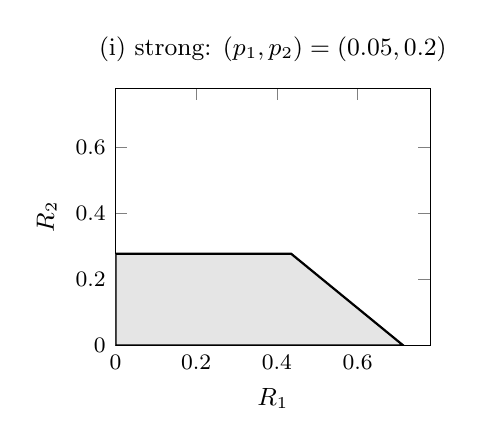
\begin{tikzpicture}
\begin{axis}[width=0.46\textwidth,height=0.4\textwidth,
  xlabel={$R_1$}, ylabel={$R_2$}, xmin=0, xmax=0.78, ymin=0, ymax=0.78,
  title={(i) strong: $(p_1,p_2)=(0.05,0.2)$},
  title style={font=\small}, label style={font=\small},
  tick label style={font=\footnotesize}]
\addplot[thick, fill=gray!20] coordinates
  {(0,0) (0,0.2781) (0.4355,0.2781) (0.7136,0) (0,0)};
\end{axis}
\end{tikzpicture}\hfill
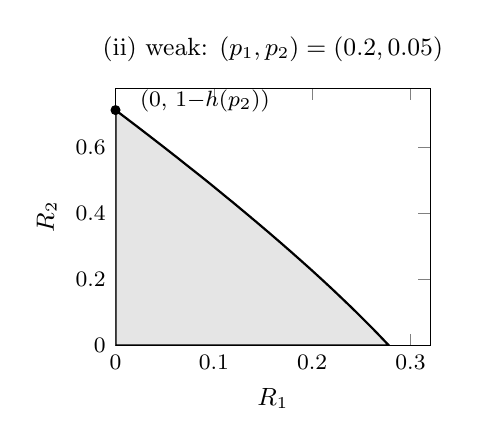
\begin{tikzpicture}
\begin{axis}[width=0.46\textwidth,height=0.4\textwidth,
  xlabel={$R_1$}, ylabel={$R_2$}, xmin=0, xmax=0.32, ymin=0, ymax=0.78,
  title={(ii) weak: $(p_1,p_2)=(0.2,0.05)$},
  title style={font=\small}, label style={font=\small},
  tick label style={font=\footnotesize}]
\addplot[thick, fill=gray!20] coordinates
  {(0,0) (0,0.7136) (0.0126,0.6851) (0.0252,0.6565) (0.0376,0.6280)
   (0.0500,0.5994) (0.0622,0.5709) (0.0743,0.5423) (0.0864,0.5138)
   (0.0983,0.4853) (0.1100,0.4567) (0.1217,0.4282) (0.1332,0.3996)
   (0.1446,0.3711) (0.1559,0.3425) (0.1670,0.3140) (0.1780,0.2854)
   (0.1888,0.2569) (0.1995,0.2284) (0.2100,0.1998) (0.2203,0.1713)
   (0.2304,0.1427) (0.2404,0.1142) (0.2501,0.0856) (0.2597,0.0571)
   (0.2690,0.0285) (0.2781,0) (0,0)};
\addplot[only marks, mark=*, mark size=1.6pt] coordinates {(0,0.7136)};
\node[font=\footnotesize, anchor=west] at (axis cs:0.015,0.74)
  {$(0,\,1{-}h(p_2))$};
\end{axis}
\end{tikzpicture}
\caption{Capacity regions of the BS-ZIC in the two regimes. Left: the
strong-interference polytope of Theorem~\ref{thm}(i). Right: the
weak-interference region of Theorem~\ref{thm}(ii); the marked corner is the
unique sum-capacity rate pair.}
\label{fig:regions}
\end{figure}

\section{Strong-Interference Regime}

\paragraph{Converse}
Suppose $p_1\le p_2$. Then $p_2=p_1\st p_0$ for some
$p_0\in[0,\tfrac12)$, so we may couple
$N_2^n=N_1^n\oplus N_0^n$, with
$N_0^n$ i.i.d. $\mathrm{Bern}(p_0)$ and independent of all other variables.
This coupling preserves the marginal channel from $X_2^n$ to $Y_2^n$ and
gives
\[
I(X_2^n;Y_2^n)
\le I(X_2^n;X_2^n\oplus N_1^n)
=I(X_2^n;Y_1^n\mid X_1^n),
\]
where the equality uses independence of the encoders and the fact that,
conditioned on $X_1^n$, adding $X_1^n$ is a bijection.

By Fano's inequality and data processing, for some $\epsilon_n\to0$,
\begin{align*}
n(R_1+R_2-\epsilon_n)
&\le I(X_1^n;Y_1^n)+I(X_2^n;Y_2^n)\\
&\le I(X_1^n;Y_1^n)+I(X_2^n;Y_1^n\mid X_1^n)\\
&=I(X_1^n,X_2^n;Y_1^n)\\
&\le n\bigl(1-h(p_1)\bigr).
\end{align*}
The point-to-point channel to receiver~2 also gives
$R_2\le1-h(p_2)$.

\paragraph{Achievability}
Choose independent uniform inputs. Receiver~1 jointly decodes both messages
on the binary additive multiple-access channel. Its achievable region is
\[
R_1\le1-h(p_1),\quad R_2\le1-h(p_1),\quad
R_1+R_2\le1-h(p_1);
\]
note that all three constraints share the same right-hand side, so
receiver~1's region is a simplex rather than the usual pentagon: the
modulo-2 sum collapses both codewords into a single binary observation.
Receiver~2 requires $R_2\le1-h(p_2)$. Since $p_1\le p_2$ implies
$1-h(p_2)\le1-h(p_1)$, the resulting achievable region matches the converse.
\hfill$\blacksquare$

\section{Weak-Interference Regime}

\paragraph{Converse}
Suppose $p_1>p_2$ and write $p_1=p_2\st q$, where
$q=(p_1-p_2)/(1-2p_2)$. Couple
$N_1^n=N_2^n\oplus Q^n$, where $Q^n$ is i.i.d.
$\mathrm{Bern}(q)$ and independent of all other variables. Let
\[
V^n=X_2^n\oplus N_2^n,
\]
so $V^n$ has the same distribution as $Y_2^n$. Fano's inequality at
receiver~2 gives
\begin{equation}\label{eq:Ventropy}
\frac1nH(V^n)\ge h(p_2)+R_2-\epsilon_n.
\end{equation}

Define
\[
f_q(t)=h\!\left(q\st h^{-1}(t)\right),\qquad 0\le t\le1.
\]
Mrs.~Gerber's Lemma~\cite{WZ73a} states that
\[
\frac1nH(V^n\oplus Q^n)\ge
f_q\!\left(\frac1nH(V^n)\right).
\]
The function $f_q$ is increasing. Hence, using~\eqref{eq:Ventropy},
Fano's inequality at receiver~1, and independence of the encoders,
\begin{align*}
R_1-\epsilon_n
&\le \frac1n I(X_1^n;Y_1^n)\\
&\le 1-\frac1nH(Y_1^n\mid X_1^n)\\
&=1-\frac1nH(V^n\oplus Q^n)\\
&\le1-f_q\!\left(h(p_2)+R_2-\epsilon_n\right).
\end{align*}
For sufficiently large $n$ the argument lies in $[0,1]$; endpoint cases
follow by continuity. Letting $n\to\infty$ proves the outer bound in
Theorem~\ref{thm}(ii).

\paragraph{Achievability}
Fix $\pi\in[0,\tfrac12]$. Let user~2 employ an i.i.d. or
constant-composition $\mathrm{Bern}(\pi)$ random code and let user~1 use a
uniform random code. Receiver~2 achieves any rate below
\[
I(X_2;Y_2)=h(\pi\st p_2)-h(p_2).
\]
Receiver~1 treats $X_2$ as noise. Since
$X_2\oplus N_1\sim\mathrm{Bern}(\pi\st p_1)$, it achieves any rate below
\[
I(X_1;Y_1)=1-h(\pi\st p_1).
\]
Set $s=\pi\st p_2$. Then
$h(s)=h(p_2)+R_2$ on the boundary, and
\[
\pi\st p_1
=\pi\st(p_2\st q)
=(\pi\st p_2)\st q
=s\st q.
\]
Therefore
\[
R_1=1-h\!\left(q\st h^{-1}(h(p_2)+R_2)\right).
\]
As $\pi$ ranges over $[0,\tfrac12]$, $s$ ranges over
$[p_2,\tfrac12]$, so this construction traces the entire outer-boundary
curve. Rates below the boundary are obtained by coding below the two mutual
informations; no time sharing is needed to trace the boundary. Moreover,
none is needed anywhere: $f_q$ is convex~\cite{WZ73a}, so the boundary curve
$R_1=1-f_q(h(p_2)+R_2)$ is concave in $R_2$ and the region is convex as
stated.

\paragraph{Unique sum-capacity rate pair}
Along the boundary, parameterized by $s\in[p_2,\tfrac12]$,
\[
R_1+R_2
=1-h(p_2)+h(s)-h(q\st s).
\]
If $s<\tfrac12$ and $q>0$, then
$s<q\st s<\tfrac12$, and therefore
$h(s)<h(q\st s)$. Thus the sum is strictly smaller than
$1-h(p_2)$ unless $s=\tfrac12$. Equality occurs only at
$(R_1,R_2)=(0,1-h(p_2))$.
\hfill$\blacksquare$

\section{Discussion}

\paragraph{No very-strong-interference regime}
In the Gaussian and general discrete interference channels, sufficiently
strong interference eventually renders the sum constraint inactive and the
capacity region becomes the interference-free rectangle. That never happens
here: both messages must be extracted from the single binary observation
$Y_1$, so $I(X_1^n,X_2^n;Y_1^n)\le n(1-h(p_1))$ caps the sum rate for
\emph{every} $p_1\le p_2$, and the interfered user pays a rate penalty no
matter how favorable its own channel. The modulo-2 collapse of the
multiple-access geometry (the simplex noted above) is the mechanism.

\paragraph{Broadcast-channel correspondence}
The weak-regime formula matches the degraded binary symmetric broadcast
channel. Under the standard superposition parameterization, user~1's
uniform codeword corresponds to the cloud-center variable carrying the
weak-receiver message, while user~2's biased codeword corresponds to the
binary satellite increment carrying the strong-receiver private message.
This is a capacity-region equivalence, not a literal equality of channel
laws: receiver~2 in~\eqref{eq:model} observes the satellite increment
directly, whereas the strong broadcast receiver would first decode the
cloud center and then recover the satellite layer. Benzel's degraded
additive-interference result~\cite{Benzel79} and the Z-channel formulation
of Liu and Goldsmith~\cite{LG09} formalize this equivalence.

\paragraph{A decode-all/TIN dichotomy}
When $p_1\le p_2$, receiver~1 can decode user~2's message at least as
reliably as receiver~2 can, once $X_1^n$ is given; full interference decoding
is optimal. When $p_1>p_2$, the entire boundary is achieved by treating
interference as noise with an optimized input bias. Thus the
Han--Kobayashi partial-decoding mechanism~\cite{HK81} is unnecessary for
this channel, although it remains fundamental for general interference
channels. This exact discrete example complements broader Gaussian
TIN-optimality results~\cite{GNAJ15}.

\paragraph{Binary versus Gaussian models}
Mrs.~Gerber's Lemma gives the exact entropy tradeoff produced by a binary
symmetric degradation, which is why the weak-regime converse closes in a
single step. No comparably tight extremal relation is known for the weak
Gaussian Z-interference geometry: there, the sum capacity in the
noisy-interference regime was settled by
\cite{ShangKramerChen09,AnnapureddyVeeravalli09,MotahariKhandani09} (with
TIN sum-optimal), while the full capacity region remains open, with recent
progress refining inner and outer bounds~\cite{Costa85,CNN24,GNZ24}. In the
binary symmetric case the entire region follows in a few lines.

\section*{Acknowledgment and AI-Use Disclosure}

Generative-AI systems were used to produce initial proof sketches and
manuscript text. A Gemini-based agent produced an early strong-interference
proof; Claude Fable~5 (Anthropic) produced an initial weak-interference
proof and draft; and GPT-5-Codex (OpenAI) was used for adversarial checking
and revision suggestions. AI-generated material affected the initial
versions of the abstract, introduction, proof sections, discussion, and
reference organization. The human authors independently checked the final
mathematical derivations, verified the cited sources, revised the wording,
and accept full responsibility for the manuscript. No AI system is listed
as an author. This disclosure is intended to comply with IEEE guidance on
AI-generated content.

\begin{thebibliography}{99}

\bibitem{WZ73a}
A.~D. Wyner and J.~Ziv, ``A theorem on the entropy of certain binary
sequences and applications---Part I,'' \emph{IEEE Trans. Inf. Theory},
vol.~19, no.~6, pp.~769--772, Nov.~1973,
doi: 10.1109/TIT.1973.1055107.

\bibitem{Wyner73b}
A.~D. Wyner, ``A theorem on the entropy of certain binary sequences and
applications---Part II,'' \emph{IEEE Trans. Inf. Theory}, vol.~19, no.~6,
pp.~772--777, Nov.~1973, doi: 10.1109/TIT.1973.1055108.

\bibitem{Carleial75}
A.~B. Carleial, ``A case where interference does not reduce capacity,''
\emph{IEEE Trans. Inf. Theory}, vol.~21, no.~5, pp.~569--570, Sep.~1975,
doi: 10.1109/TIT.1975.1055432.

\bibitem{Sato78}
H.~Sato, ``On the capacity region of a discrete two-user channel for strong
interference,'' \emph{IEEE Trans. Inf. Theory}, vol.~24, no.~3,
pp.~377--379, May 1978.

\bibitem{Benzel79}
R.~Benzel, ``The capacity region of a class of discrete additive degraded
interference channels,'' \emph{IEEE Trans. Inf. Theory}, vol.~25, no.~2,
pp.~228--231, Mar.~1979, doi: 10.1109/TIT.1979.1056025.

\bibitem{HK81}
T.~S. Han and K.~Kobayashi, ``A new achievable rate region for the
interference channel,'' \emph{IEEE Trans. Inf. Theory}, vol.~27, no.~1,
pp.~49--60, Jan.~1981, doi: 10.1109/TIT.1981.1056307.

\bibitem{Sato81}
H.~Sato, ``The capacity of the Gaussian interference channel under strong
interference,'' \emph{IEEE Trans. Inf. Theory}, vol.~27, no.~6,
pp.~786--788, Nov.~1981, doi: 10.1109/TIT.1981.1056416.

\bibitem{EGC82}
A.~El~Gamal and M.~H.~M. Costa, ``The capacity region of a class of
deterministic interference channels,'' \emph{IEEE Trans. Inf. Theory},
vol.~28, no.~2, pp.~343--346, Mar.~1982.

\bibitem{Costa85}
M.~H.~M. Costa, ``On the Gaussian interference channel,'' \emph{IEEE Trans.
Inf. Theory}, vol.~31, no.~5, pp.~607--615, Sep.~1985,
doi: 10.1109/TIT.1985.1057085.

\bibitem{CEG87}
M.~H.~M. Costa and A.~El~Gamal, ``The capacity region of the discrete
memoryless interference channel with strong interference,'' \emph{IEEE
Trans. Inf. Theory}, vol.~33, no.~5, pp.~710--711, Sep.~1987,
doi: 10.1109/TIT.1987.1057340.

\bibitem{LU08}
N.~Liu and S.~Ulukus, ``The capacity region of a class of discrete degraded
interference channels,'' \emph{IEEE Trans. Inf. Theory}, vol.~54, no.~9,
pp.~4372--4378, Sep.~2008.

\bibitem{ShangKramerChen09}
X.~Shang, G.~Kramer, and B.~Chen, ``A new outer bound and the
noisy-interference sum-rate capacity for Gaussian interference channels,''
\emph{IEEE Trans. Inf. Theory}, vol.~55, no.~2, pp.~689--699, Feb.~2009.

\bibitem{MotahariKhandani09}
A.~S. Motahari and A.~K. Khandani, ``Capacity bounds for the Gaussian
interference channel,'' \emph{IEEE Trans. Inf. Theory}, vol.~55, no.~2,
pp.~620--643, Feb.~2009.

\bibitem{AnnapureddyVeeravalli09}
V.~S. Annapureddy and V.~V. Veeravalli, ``Gaussian interference networks:
Sum capacity in the low-interference regime and new outer bounds on the
capacity region,'' \emph{IEEE Trans. Inf. Theory}, vol.~55, no.~7,
pp.~3032--3050, Jul.~2009.

\bibitem{LG09}
N.~Liu and A.~J. Goldsmith, ``Capacity regions and bounds for a class of
Z-interference channels,'' \emph{IEEE Trans. Inf. Theory}, vol.~55, no.~11,
pp.~4986--4994, Nov.~2009, doi: 10.1109/TIT.2009.2030490.

\bibitem{EGK11}
A.~El~Gamal and Y.-H. Kim, \emph{Network Information Theory}. Cambridge,
U.K.: Cambridge Univ. Press, 2011.

\bibitem{GNAJ15}
C.~Geng, N.~Naderializadeh, A.~S. Avestimehr, and S.~A. Jafar, ``On the
optimality of treating interference as noise,'' \emph{IEEE Trans. Inf.
Theory}, vol.~61, no.~4, pp.~1753--1767, Apr.~2015,
doi: 10.1109/TIT.2015.2408342.

\bibitem{CNN24}
M.~H.~M. Costa, C.~Nair, and D.~Ng, ``Critical points in the Noiseberg
achievable region of the Gaussian Z-interference channel,'' \emph{Entropy},
vol.~26, no.~11, Art.~no.~898, Nov.~2024,
doi: 10.3390/e26110898.

\bibitem{GNZ24}
A.~Gohari, C.~Nair, and J.~Zhao, ``On the capacity region of some classes of
interference channels,'' in \emph{Proc. IEEE Int. Symp. Inf. Theory
(ISIT)}, 2024, pp.~3136--3141,
doi: 10.1109/ISIT57864.2024.10619605.

\end{thebibliography}

\end{document}
